% !TEX program = pdflatex
\documentclass[10pt]{article}

% =========================
% Basics / Layout
% =========================
\usepackage[T1]{fontenc} % 8-bit encoding
\usepackage{geometry}
\geometry{margin=1in}

% =========================
% Fonts (from your HW)
% =========================
\renewcommand{\rmdefault}{ptm}
\usepackage{mathptmx}

% =========================
% Math / Theorems (from your HW)
% =========================
\usepackage{amsmath,amsthm,amsfonts,amssymb,mathtools}
\usepackage{bm}
\usepackage{dsfont}
\usepackage{xparse}
\usepackage[mathscr]{euscript}
\usepackage[super]{nth}

% =========================
% General utilities (from your HW)
% =========================
\usepackage{enumitem,wrapfig,graphicx}
\usepackage{sectsty}
\usepackage{xcolor}
\definecolor{darkpastelgreen}{rgb}{0.01, 0.75, 0.24}
\definecolor{blue-violet}{rgb}{0.54, 0.17, 0.89}

% =========================
% TikZ/PGFPlots (from your HW)
% =========================
\usepackage{pgfplots}
\pgfplotsset{compat=1.18}
\usetikzlibrary{arrows.meta}
\usepackage{float}
\usetikzlibrary{matrix}

% =========================
% Polynomial tools (from your HW)
% =========================
\usepackage{polynom}

% =========================
% Spacing (from your HW)
% =========================
\usepackage{parskip}
\usepackage{setspace}

%\doublespacing

% ============================================================
% Your custom environments + theorem setup (from your HW)
% ============================================================
\newcounter{cprob}
\newenvironment{cprob}[1]{%
    \setcounter{cprob}{#1}%
    \noindent\textbf{Problem \thecprob.}%
}{%
    \par\bigskip%
}

\theoremstyle{plain}
\newcommand{\theoremname}{Theorem}
\newtheorem{thm}{\protect\theoremname}
\theoremstyle{definition}
\newtheorem{prob}[thm]{Problem}
\newtheorem*{problem*}{Open Problem}
\theoremstyle{plain}
\newtheorem{conjecture}[thm]{Conjecture}
\newtheorem{lem}[thm]{Lemma}
\newtheorem*{lem*}{Lemma}
\newtheorem{obs}[thm]{Observation}
\newtheorem{cor}[thm]{Corollary}
\theoremstyle{definition}
\newtheorem{definition}[thm]{Definition}

% Patch prob to be single spaced (requires setspace; you already have it)
\let\oldprob\prob
\let\endoldprob\endprob
\renewenvironment{prob}
  {\begin{singlespace}\oldprob}
  {\endoldprob\end{singlespace}}

% ============================================================
% Your macros (from your HW)
% ============================================================
\newcommand{\belowtitle}{\leavevmode\newline}
\newcommand{\Observe}{\text{Observe.}}
\newcommand{\IF}{\mathbf{(\Rightarrow)}}
\newcommand{\FI}{\mathbf{(\Leftarrow)}}
\newcommand{\class}[2][]{\ensuremath{\left[\,#2\,\right]_{#1}}}

\newcommand{\horrule}[1]{\rule{\linewidth}{#1}}
\newcommand{\kkk}{\ensuremath{\Bbbk}}
\newcommand{\CC}{\ensuremath{\mathbb{C}}}
\newcommand{\FF}{\ensuremath{\mathbb{F}}}
\newcommand{\KK}{\ensuremath{\mathbb{K}}}
\newcommand{\NN}{\ensuremath{\mathbb{N}}}
\newcommand{\QQ}{\ensuremath{\mathbb{Q}}}
\newcommand{\RR}{\ensuremath{\mathbb{R}}}
\newcommand{\ZZ}{\ensuremath{\mathbb{Z}}}
\newcommand{\MM}{\ensuremath{\mathcal{M}}}
\newcommand{\GG}{\ensuremath{\mathcal{G}}}
\newcommand{\TT}{\ensuremath{\mathcal{T}}}
\newcommand{\BB}{\ensuremath{\mathcal{B}}}
\newcommand{\VV}{\ensuremath{\mathcal{V}}}
\newcommand{\WW}{\ensuremath{\mathcal{W}}}
\newcommand{\UU}{\ensuremath{\mathcal{U}}}
\newcommand{\PP}{\ensuremath{\mathcal{P}}}
\newcommand{\LL}{\ensuremath{\mathcal{L}}}
\newcommand{\kk}{\ensuremath{\mathds{k}}}
\newcommand{\EE}{\ensuremath{\mathbb{E}}}

\newcommand{\sm}{\char`\\}

\DeclarePairedDelimiter{\ip}{\langle}{\rangle}
\DeclarePairedDelimiter{\norm}{\lVert}{\rVert}
\DeclarePairedDelimiter{\sqb}{\lbrack}{\rbrack}
\newcommand{\floor}[1]{\left\lfloor #1 \right\rfloor}
\newcommand{\ceil}[1]{\left\lceil #1 \right\rceil}
\newcommand{\mbf}[1]{\ensuremath{\mathbf{#1}}}
\newcommand{\tbf}[1]{\textbf{ #1 }}
\newcommand{\Span}{\ensuremath{\mathrm{Span}}}
\newcommand{\Char}[1]{\mathrm{Char}\; #1}
\DeclareMathOperator{\lcm}{lcm}
\newcommand{\id}{\ensuremath{\mathrm{id}}}
\newcommand{\Gal}[2]{\mathrm{Gal}(#1/#2)}
\newcommand{\Aut}{\ensuremath{\mathrm{Aut}}}
\newcommand{\Fix}[2]{\mathrm{Fix}_{#1}(#2)}
\newcommand{\proj}[2]{\text{proj}_{#1}(#2)}

% keep your matrix spacing patches
\makeatletter
\renewcommand*\env@matrix[1][*\c@MaxMatrixCols c]{%
  \hskip -\arraycolsep
  \let\@ifnextchar\new@ifnextchar
  \array{#1}}
\makeatother
\def\env@matrix{\hskip -\arraycolsep
  \let\@ifnextchar\new@ifnextchar
  \array{*\c@MaxMatrixCols c}}

% Your re-declare (kept)
\DeclareMathAlphabet{\mathcal}{OMS}{cmsy}{m}{n}

% ============================================================
% Title info (paper-style)
% ============================================================
\usepackage{fancyhdr}
\pagestyle{fancy}
\fancyhf{}
\renewcommand{\headrulewidth}{0pt} % no line

\fancypagestyle{titlepage}{
  \fancyhf{}
  \fancyhead[L]{Danny Banegas}
  \fancyhead[R]{\today}
}

\title{Decompositions of Complete Graphs}
\makeatletter
\renewcommand{\maketitle}{
  \begin{center}
    {\LARGE \@title \par}
  \end{center}
}
\makeatother

\begin{document}
\maketitle

\thispagestyle{titlepage}
\begin{center}
A write-up on, \textit{Seven Edge Forest Designs}, by Daniel Banegas and Professor Bryan Freyberg of UMN Duluth
\end{center}
\section{Introduction}
Suppose you have $n$ translucent sheets of tracing paper with some points drawn on all $n$ sheets of paper in the same set arrangement. Now, draw lines connecting points on each sheet of paper, so that no line appears on two distinct sheets of paper.

A graph $K$ is depicted when all $n$ sheets of tracing paper are aligned and stacked on top of each other with some light source present. Call the graph depicted on the $i$th sheet of paper $G_{i}$ for $i=1,\hdots,n$. The stacking of these sheets of paper depicts the edge-disjoint union $G_{1}\cup \cdots \cup G_{n}=K$, and this collection of papers depicts the set $\{G_{1},\hdots,G_{n}\}$ which we call a \textit{graph decomposition} of $K$. This is defined formally below.

\begin{definition}[Graph Decomposition]
Let $K$ be a simple graph. We call a collection $\{G_{1},\hdots,G_{n}\}$ of pairwise edge-disjoint subgraphs $G_{1},\hdots,G_{n}\subseteq K$ of $K$ a \textit{decomposition} of $K$ if their union equals $K$.
\end{definition}
\begin{figure}[H]
  \begin{center}
      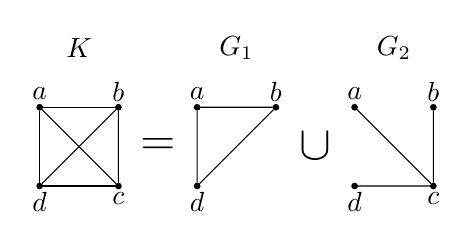
\begin{tikzpicture}[every node/.style={draw, circle, fill=black, minimum size=2pt, inner sep=0pt}]
          % First Graph
          \node (T)[draw=none, fill=none] at (0.5,0.75) {$K$};
          \node (0) at (0, 0)[label=above:$a$]  {};
          \node (1) at (1, 0)[label=above:$b$]  {};
          \node (2) at (1, -1)[label=below:$c$] {};
          \node (3) at (0, -1)[label=below:$d$] {};

          \draw (2) -- (3) -- (0) -- (1);
          \draw (0) -- (2) -- (1) -- (3);
          % "=" symbol
          \node[draw=none, fill=none] at (1.5, -0.5) {\LARGE $=$};

          % Second graph
          \begin{scope}[xshift=2cm]
            \node (T)[draw=none, fill=none] at (0.5,0.75) {$G_{1}$};
            \node (0) at (0, 0)[label=above:$a$]  {};
            \node (1) at (1, 0)[label=above:$b$]  {};
            \node (3) at (0, -1)[label=below:$d$] {};

              \draw (0) -- (1) -- (3) -- (0);
          \end{scope}
          
          % "\cup" symbol
          \node[draw=none, fill=none] at (3.5, -0.5) {\LARGE $\cup$};
          
          \begin{scope}[xshift=4cm]
            \node (T)[draw=none, fill=none] at (0.5,0.75) {$G_{2}$};
            \node (0) at (0, 0)[label=above:$a$]  {};
            \node (1) at (1, 0)[label=above:$b$]  {};
            \node (2) at (1, -1)[label=below:$c$] {};
            \node (3) at (0, -1)[label=below:$d$] {};
              
            \draw (3) -- (2) -- (0) -- (2) -- (1);
          \end{scope}
      \end{tikzpicture}
  \end{center}
  \caption{[1] $\{G_{1},G_{2}\}$ is a decomposition of $K_{4}$.}
  \label{fig:simpledecompex}
\end{figure}
If all the graphs in a decomposition $\GG=\{G_{1},\hdots, G_{m}\}$ of $K$ are isomorphic to some graph $G$, then we call $\GG$ a $G$-decomposition of $K$ or a $(K,G)$-design, and if $K$ is isomorphic to the complete graph $K_{n}$ we say $\GG$ is a $G$-design of order $n$. Once again, we define this formally below.

\begin{definition}[$G$-decomposition]
A \textit{$G$-decomposition} of a graph $K$ is a decomposition $\{G_{1},\hdots,G_{t}\}$ of $K$ whose members are all isomorphic to some graph $G$. If such a set exists we say that $K$ \textit{allows} a $G$-decomposition or equivalently, that $G$ \textit{decomposes} $K$. If $K\cong K_{n}$ we sometimes call the decomposition a \textit{$G$-design of order $n$}.
\end{definition}

\begin{figure}[H]
  \begin{center}
      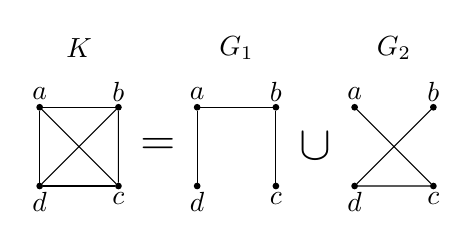
\begin{tikzpicture}[every node/.style={draw, circle, fill=black, minimum size=2pt, inner sep=0pt}]
          % First Graph
          \node (T)[draw=none, fill=none] at (0.5,0.75) {$K$};
          \node (0) at (0, 0)[label=above:$a$]  {};
          \node (1) at (1, 0)[label=above:$b$]  {};
          \node (2) at (1, -1)[label=below:$c$] {};
          \node (3) at (0, -1)[label=below:$d$] {};

          \draw (2) -- (3) -- (0) -- (1);
          \draw (0) -- (2) -- (1) -- (3);
          % "=" symbol
          \node[draw=none, fill=none] at (1.5, -0.5) {\LARGE $=$};

          % Second graph
          \begin{scope}[xshift=2cm]
            \node (T)[draw=none, fill=none] at (0.5,0.75) {$G_{1}$};
            \node (0) at (0, 0)[label=above:$a$]  {};
            \node (1) at (1, 0)[label=above:$b$]  {};
            \node (2) at (1, -1)[label=below:$c$] {};
            \node (3) at (0, -1)[label=below:$d$] {};

              \draw (3) -- (0) -- (1) -- (2);
          \end{scope}
          
          % "\cup" symbol
          \node[draw=none, fill=none] at (3.5, -0.5) {\LARGE $\cup$};
          
          \begin{scope}[xshift=4cm]
            \node (T)[draw=none, fill=none] at (0.5,0.75) {$G_{2}$};
            \node (0) at (0, 0)[label=above:$a$]  {};
            \node (1) at (1, 0)[label=above:$b$]  {};
            \node (2) at (1, -1)[label=below:$c$] {};
            \node (3) at (0, -1)[label=below:$d$] {};
              
            \draw (0) -- (2) -- (3) -- (1);
          \end{scope}
      \end{tikzpicture}
  \end{center}
  \caption{[1] $\{G_{1},G_{2}\}$ is a $P_{3}$-decomposition of $K_{4}$ or a $P_{3}$-design of order $4$.}
  \label{fig:Gdecompex}
\end{figure}

\section{Existence}
If a $G$-decomposition of some graph $K$ exists, then all of its members have the same number of edges and vertices. This allows us to find constraints on graphs $K$ that can be decomposed by some subgraph $G\subseteq K$ on $m$ edges solely based on divisiblity properties.

\begin{lem}[Necessary Condition (general)] \label{lem:gencondition}
  Let $G$ be a simple graph on $m$ edges. There exists a $G$-decomposition of a graph $K$ only if $m$ divides $|E(K)|$. 
\end{lem}

  \begin{proof}
  Suppose there exists a $G$-decomposition $\{G_{1},\hdots, G_{n}\}$ of $K$. Then $E(G_{1})\sqcup \cdots \sqcup\,E(G_{t})=E(K)$ and so $|E(K)|=|E(G_{1})\sqcup \cdots \sqcup E(G_{t})|=|E(G_{1})|+ \cdots + |E(G_{t})|=tm$. So $|E(G)|=m$ divides $|E(K)|$.
  \end{proof}

\begin{thm}[Necessary Condition ($K_{n}$)] \label{thm:Kncondition}
  Let $G$ be a simple graph on $m$ edges. There exists a $G$-decomposition of $K_{n}$ only if $n$ is idempotent modulo $2m$, that is, only if $n^{2}\equiv n\pmod{2m}$.
\end{thm}
\begin{proof}
  Suppose there exists a $G$-decomposition of $K_{n}$. Then $|E(G)|=m$ divides $|E(K_{n})|=\binom{n}{2}=\frac{n(n-1)}{2}$ by Lemma \ref{lem:gencondition}. Therefore, $\frac{n^{2}-n}{2}=mt$ for some $t\in \NN$. Observe
  $$n^{2}-n= 2mt\implies n^{2}-n\equiv 0\pmod{2m}\implies n^{2}\equiv n\pmod{2m}.$$
\end{proof}
By the previous theorem, any graph on $m$ edges decomposes $K_{n}$ only if $n$ is idempotent modulo $2m$. Note that the converse is not necessarily true. However, for a graph $G$ on $m$ edges, this finite set of constraints allows us to ask:
\begin{center}
For what $n$ is $K_{n}$ $G$-decomposable?
\end{center}
This question is known as the \textit{spectrum problem} for graph decompositions. Pioneering work by Rosa and Kotzig in the 1960s, especially in the development of \textit{graph labelings}, helped shape the modern approach to $G$-decomposition problems.

Let's put everything together. Suppose $G$ is a graph on $m$ edges, and that you want to find all complete graphs $K_{n}$ that are $G$-decomposable. By some previous theorems, we have that $n$ must be idempotent modulo $2m$. Well, there are only finitely many idempotents $r$, two of which are always $0$ and $1$, in the cyclic ring $\ZZ_{2m}$ for any particular $m$. So then if we prove that $G$ decomposes (or that it doesn't decompose) $K_{2mt+r}$ for all $t\geq 1$ and all idempotents $r\in \ZZ_{2m}$, we get necessary and sufficient conditions for the existence of a $G$-design of order $n$. 

\section{Intuition}
Before discussing labelings formally, we take a peek beneath the hood. Often the definitions of labelings and then their subsequent results are presented and justified in a very terse manner. However, the intuition behind them is actually very simple. Let's begin with an example.

Take the vertices of $K_{5}$ to be $\ZZ_{5}$, and draw it so that it looks like a Pentagram where the vertices appear in increasing order along the outer cycle. Notice that every vertex shares an edge with two vertices directly adjacent to it and two vertices that are `two adjacencies away' on the outer cycle $(01234)$. We say two vertices $u,v$ have \textit{length} $\ell(uv)=l$ if they are `$l$ adjacencies away' from each other on the outer cycle. Color length $1$ edges \textcolor{blue}{blue} and length $2$ edges \textcolor{red}{red}.
\begin{figure}[H]
  \begin{center}
  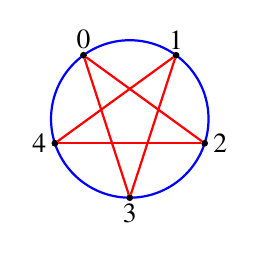
\begin{tikzpicture}[scale=1, every node/.style={draw, circle, fill=black, minimum size=2pt, inner sep=0pt}]
  
  % Outer circle in blue
  \draw[blue, thick] (0,0) circle (1);
  
  % Place nodes on the circle
  \node (0) at (126:1) [label=above:0]{};   % upper left
  \node (1) at (54:1)  [label=above:1]{};   % upper right
  \node (2) at (342:1) [label=right:2]{};   % lower right
  \node (3) at (270:1) [label=below:3]{};   % bottom
  \node (4) at (198:1) [label=left:4]{};   % lower left

  % Internal edges (diagonals) in red
  \draw[red, thick] (0) -- (2);
  \draw[red, thick] (1) -- (3);
  \draw[red, thick] (2) -- (4);
  \draw[red, thick] (3) -- (0);
  \draw[red, thick] (4) -- (1);
  
  \end{tikzpicture}
  \end{center}
  \caption{[1] $K_{5}$ with lengths colored.}
  \label{fig:K5colored}
\end{figure}
Notice that this gives a partition of $E(K_{5})$, whose partite sets are of equal size $5$. Now, consider $P_{3}$. It has $2$ edges, and $K_{5}$ has $\binom{5}{2}=10$ edges. Since $2|10$, by Lemma \ref{lem:gencondition} it's \textit{possible} that a $P_{3}$-decomposition of $K_{5}$ exists. Well, since $P_{3}$ has $2$ edges and there are $2$ possible lengths in $K_{5}$, we can form copies of $P_{3}$ that has both a \textcolor{blue}{blue} edge and a \textcolor{red}{red} edge. It turns out that we can generate all these copies from just one subgraph of $K_{n}$, if we are clever about the subgraph we choose, by permuting it's vertices repeatedly.
\begin{figure}[H]
  \begin{center}
  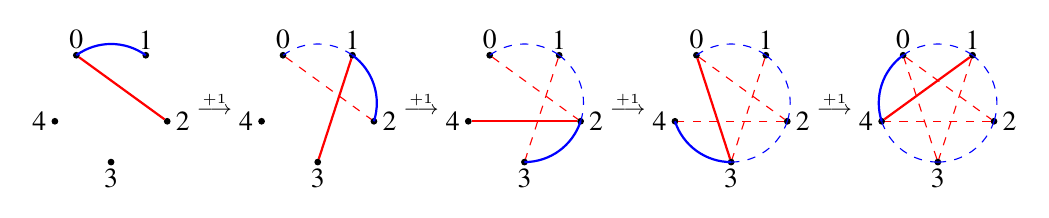
\begin{tikzpicture}[scale=0.75, every node/.style={draw, circle, fill=black, minimum size=2pt, inner sep=0pt}]
  
  % Outer circle in blue
  %\draw[blue, thick] (0,0) circle (1);

  % (2,0,1)
  % Place nodes on the circle
  \node (0) at (126:1) [label=above:0]{};   % upper left
  \node (1) at (54:1)  [label=above:1]{};   % upper right
  \node (2) at (342:1) [label=right:2]{};   % lower right
  \node (3) at (270:1) [label=below:3]{};   % bottom
  \node (4) at (198:1) [label=left:4]{};   % lower left
      
  %Draw the outer cycle edges as arcs along the circle
  %\draw[blue, thick] (3) arc (270:342:1); %3 -- 2
  %\draw[blue, thick] (2) arc (342:414:1); %2 -- 1 
  \draw[blue, thick] (1) arc (54:126:1);  %1 -- 0
  %\draw[blue, thick] (0) arc (126:198:1); %0 -- 4
  %\draw[blue, thick] (4) arc (198:270:1); %4 -- 3

  % Internal edges (diagonals) in red
  \draw[red, thick] (0) -- (2);
  %\draw[red, thick] (1) -- (3);
  %\draw[red, thick] (2) -- (4);
  %\draw[red, thick] (3) -- (0);
  %\draw[red, thick] (4) -- (1);
  \node[draw=none, fill=none] at (1.75, 0) {\scriptsize $\overset{+1}{\longrightarrow}$};

  \begin{scope}[shift={(3.5,0)}]
    %(3,1,2)
    \node (0) at (126:1) [label=above:0]{};   % upper left
    \node (1) at (54:1)  [label=above:1]{};   % upper right
    \node (2) at (342:1) [label=right:2]{};   % lower right
    \node (3) at (270:1) [label=below:3]{};   % bottom
    \node (4) at (198:1) [label=left:4]{};   % lower left
        
    %Draw the outer cycle edges as arcs along the circle
    %\draw[blue, thick] (3) arc (270:342:1); %3 -- 2
    \draw[blue, thick] (2) arc (342:414:1); %2 -- 1 
    \draw[blue, dashed] (1) arc (54:126:1);  %1 -- 0
    %\draw[blue, thick] (0) arc (126:198:1); %0 -- 4
    %\draw[blue, thick] (4) arc (198:270:1); %4 -- 3

    % Internal edges (diagonals) in red
    \draw[red, dashed] (0) -- (2);
    \draw[red, thick] (1) -- (3);
    %\draw[red, thick] (2) -- (4);
    %\draw[red, thick] (3) -- (0);
    %\draw[red, thick] (4) -- (1);
    \node[draw=none, fill=none] at (1.75, 0) {\scriptsize $\overset{+1}{\longrightarrow}$};
  \end{scope}

  \begin{scope}[shift={(7,0)}]
    %(4,2,3)
    \node (0) at (126:1) [label=above:0]{};   % upper left
    \node (1) at (54:1)  [label=above:1]{};   % upper right
    \node (2) at (342:1) [label=right:2]{};   % lower right
    \node (3) at (270:1) [label=below:3]{};   % bottom
    \node (4) at (198:1) [label=left:4]{};   % lower left
        
    %Draw the outer cycle edges as arcs along the circle
    \draw[blue, thick] (3) arc (270:342:1); %3 -- 2
    \draw[blue, dashed] (2) arc (342:414:1); %2 -- 1 
    \draw[blue, dashed] (1) arc (54:126:1);  %1 -- 0
    %\draw[blue, thick] (0) arc (126:198:1); %0 -- 4
    %\draw[blue, thick] (4) arc (198:270:1); %4 -- 3

    % Internal edges (diagonals) in red
    \draw[red, dashed] (0) -- (2);
    \draw[red, dashed] (1) -- (3);
    \draw[red, thick] (2) -- (4);
    %\draw[red, thick] (3) -- (0);
    %\draw[red, thick] (4) -- (1);
    \node[draw=none, fill=none] at (1.75, 0) {\scriptsize $\overset{+1}{\longrightarrow}$};
  \end{scope}

  \begin{scope}[shift={(10.5,0)}]
    %(0,3,4)
    \node (0) at (126:1) [label=above:0]{};   % upper left
    \node (1) at (54:1)  [label=above:1]{};   % upper right
    \node (2) at (342:1) [label=right:2]{};   % lower right
    \node (3) at (270:1) [label=below:3]{};   % bottom
    \node (4) at (198:1) [label=left:4]{};   % lower left
        
    %Draw the outer cycle edges as arcs along the circle
    \draw[blue, dashed] (3) arc (270:342:1); %3 -- 2
    \draw[blue, dashed] (2) arc (342:414:1); %2 -- 1 
    \draw[blue, dashed] (1) arc (54:126:1);  %1 -- 0
    %\draw[blue, thick] (0) arc (126:198:1); %0 -- 4
    \draw[blue, thick] (4) arc (198:270:1); %4 -- 3

    % Internal edges (diagonals) in red
    \draw[red, dashed] (0) -- (2);
    \draw[red, dashed] (1) -- (3);
    \draw[red, dashed] (2) -- (4);
    \draw[red, thick] (3) -- (0);
    %\draw[red, thick] (4) -- (1);
    \node[draw=none, fill=none] at (1.75, 0) {\scriptsize $\overset{+1}{\longrightarrow}$};
  \end{scope}
  \begin{scope}[shift={(14,0)}]
    %(1,4,0)
    \node (0) at (126:1) [label=above:0]{};   % upper left
    \node (1) at (54:1)  [label=above:1]{};   % upper right
    \node (2) at (342:1) [label=right:2]{};   % lower right
    \node (3) at (270:1) [label=below:3]{};   % bottom
    \node (4) at (198:1) [label=left:4]{};   % lower left
        
    %Draw the outer cycle edges as arcs along the circle
    \draw[blue, dashed] (3) arc (270:342:1); %3 -- 2
    \draw[blue, dashed] (2) arc (342:414:1); %2 -- 1 
    \draw[blue, dashed] (1) arc (54:126:1);  %1 -- 0
    \draw[blue, thick] (0) arc (126:198:1); %0 -- 4
    \draw[blue, dashed] (4) arc (198:270:1); %4 -- 3

    % Internal edges (diagonals) in red
    \draw[red, dashed] (0) -- (2);
    \draw[red, dashed] (1) -- (3);
    \draw[red, dashed] (2) -- (4);
    \draw[red, dashed] (3) -- (0);
    \draw[red, thick] (4) -- (1);
  \end{scope}
  
  \end{tikzpicture}
  \end{center}
  \caption{[1] A cyclic $P_{3}$-decomposition of $K_{5}$.}
  \label{fig:P3K5colordecomp}
\end{figure}
If $S(G)$ denotes the set of all subgraphs $K$, let $$\ZZ_{5} \curvearrowright S(K_{5})\text{ via }i(G)\coloneq (V(G),E(G))\mapsto (V(G)+i,E(G)+ii),\,\forall G\in S(K_{5})\text{ and }\forall i\in \ZZ_{5}.$$ This action is actually very simple. We just take our labeled subgraph, and add $i\in \ZZ_{5}$ to all of it's nodes at the same time, without touching the edges. We call the act of permuting all vertices of a labeling by $i$ \textit{developing} or \textit{clicking}. 

\textbf{Figure 4} depicts $\mathrm{Orb}(P)$, which can be obtained by developing $P$ by $1$ repeatedly, and where $P$ is the leftmost graph we begin with in \textbf{Figure 4}. We call a decomposition that can be generated by one subgraph in this manner a \textit{cyclic decomposition}. A lot of detail has been omitted here for the sake of developing the core intuition behind graph labelings. It doesn't always turn out this nicely, but the approach shown here can be generalized, extended, and refined to prove the existence of $G$-decompositions for infinite families of complete graphs. Before coninuing onto the next section we generalize this notion of length.

Formally, for $K_{n}$ whose vertices we take to be $\ZZ_{n}$ we define the edge length function $\ell$ as follows:
$$\ell_{n}(u,v)=\ell_{n}(v,u)=\ell_{n}(uv)=\min\{|u-v|,n-|u-v|\}.$$
\section{$\sigma^{+-}$-Labelings}
In our example, we only wanted to decompose $K_{5}$, but what about the rest of the family $K_{4t+1}$ where $t>1$? A single labeling can take care of the entire family, if it is tuned and refined properly.
\begin{definition}[Freyberg, Tran] \label{def:sigma plus minus} 
A $\sigma^{+-}$-\emph{labeling} of a bipartite graph $G$ with $m$ edges is an injection $$f:\{0,1,\hdots, 2m-2\}\to V(G)$$ such that $f(V(G))=A\sqcup B\subset V(K_{2m})$ where
\begin{align}
& uv \in f(E(G))\implies (u,v)\in A\times B\text{ or }(v,u)\in B\times A\\
& \ell_{n}(ab)=|a-b|=b-a,\forall a\in A,b\in B\\
& ab\in f(E(G))\implies a<b, \forall a\in A,\forall b\in B\\
& a-b\neq m,\forall a\in A,\forall b\in B 
\end{align}
\end{definition}
If an edge is incident to a leaf (a degree 1 vertex), we call it a \textit{pendant edge}.
\begin{thm}[Freyberg, Tran] \label{thm:sigma plus minus}
Let $G$ be a graph with $m$ edges and a $\sigma^{+-}$-labeling such that the edge of length $m$ is a pendant. Then there exists a $G$-decomposition of both $K_{2mt}$ and $K_{2mt+1}$ for every positive integer $t$.
\end{thm}

  \begin{figure}[H]
    \begin{center}
      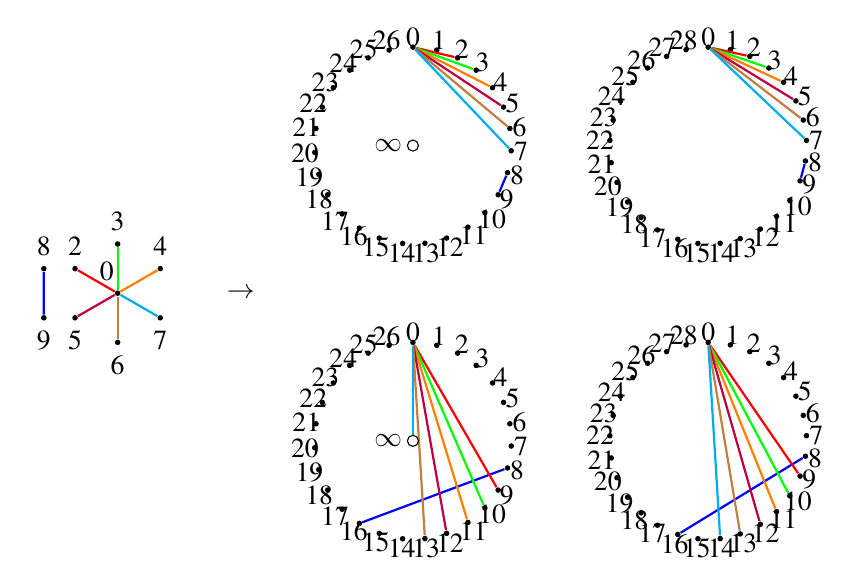
\begin{tikzpicture}[scale=1.25]
        \tikzset{
          dot/.style={circle, fill=black, minimum size=2pt, inner sep=0pt},
          infdot/.style={circle, draw=black, fill=white, minimum size=4pt, inner sep=0pt},
          lbl/.style={draw=none, fill=none, inner sep=0pt, anchor=center}
        }
  
        % — K_{29} labeling —
        \foreach \i in {0,...,28} {
          \pgfmathtruncatemacro{\angle}{90 - \i*360/29}
          \node[dot] (n\i) at (\angle:1) {};
          \node[lbl] at (\angle:1.1) {\i};
        }
        % forest on K29: path (8,9), star at 0→{2,3,4,5,6,7}
        \draw[blue,   thick] (n8) -- (n9);
        \draw[red,    thick] (n0) -- (n2);
        \draw[green,  thick] (n0) -- (n3);
        \draw[orange, thick] (n0) -- (n4);
        \draw[purple, thick] (n0) -- (n5);
        \draw[brown,  thick] (n0) -- (n6);
        \draw[cyan,   thick] (n0) -- (n7);
  
        % — K_{27} ∪ {∞} labeling (shift left) —
        \begin{scope}[shift={(-3,0)}]
          \foreach \i in {0,...,26} {
            \pgfmathtruncatemacro{\angle}{90 - \i*360/27}
            \node[dot] (m\i) at (\angle:1) {};
            \node[lbl] at (\angle:1.1) {\i};
          }
          \coordinate (inf) at (0,0);
          \draw[blue, thick] (m8) -- (m9);
          \draw[red,   thick] (m0) -- (m2);
          \draw[green, thick] (m0) -- (m3);
          \draw[orange,thick] (m0) -- (m4);
          \draw[purple,thick] (m0) -- (m5);
          \draw[brown, thick] (m0) -- (m6);
          \draw[cyan,  thick] (m0) -- (m7);
          \node[infdot] at (inf) {};
          \node[lbl]    at (-0.25,0) {$\infty$};
        \end{scope}
  
        % — K_{15} labeling (further shift left) —
        \begin{scope}[shift={(-6,-1.5)}]
          \node[dot,label=above:3] (a3) at (90:0.5)   {};
          \node[dot,label=above:4] (a4) at (30:0.5)   {};
          \node[dot,label=below:7] (a7) at (330:0.5)  {};
          \node[dot,label=below:6] (a6) at (270:0.5)  {};
          \node[dot,label=below:5] (a5) at (210:0.5)  {};
          \node[dot,label=above:2] (a2) at (150:0.5)  {};
          \node[dot,label={[xshift=3pt]above left:0}] (a0) at (0,0) {};
          \node[dot,label=above:8] (a8) at (-0.75,0.25) {};
          \node[dot,label=below:9] (a9) at (-0.75,-0.25){};
          \draw[blue,   thick] (a8) -- (a9);
          \draw[green, thick] (a0) -- (a3);
          \draw[orange,thick] (a0) -- (a4);
          \draw[cyan,  thick] (a0) -- (a7);
          \draw[brown, thick] (a0) -- (a6);
          \draw[purple,thick] (a0) -- (a5);
          \draw[red,    thick] (a0) -- (a2);
          \node[draw=none, fill=none] at (1.25, 0) {$\LARGE \rightarrow$};
        \end{scope}
  %--------------------------------------------row 2------------------------------------------------------------
      \begin{scope}[shift={(-3,-3)}]
        \foreach \i in {0,...,26} {
          \pgfmathtruncatemacro{\angle}{90 - \i*360/27}
          \node[dot] (m\i) at (\angle:1) {};
          \node[lbl] at (\angle:1.1) {\i};
        }
        \coordinate (inf) at (0,0);
        \draw[blue, thick] (m8) -- (m16);
        \draw[red,   thick] (m0) -- (m9);
        \draw[green, thick] (m0) -- (m10);
        \draw[orange,thick] (m0) -- (m11);
        \draw[purple,thick] (m0) -- (m12);
        \draw[brown, thick] (m0) -- (m13);
        \draw[cyan,  thick] (m0) -- (inf);
        \node[infdot] at (inf) {};
        \node[lbl]    at (-0.25,0) {$\infty$};
      \end{scope}

      % — K_{29} labeling —
      \begin{scope}[shift={(0,-3)}]
        \foreach \i in {0,...,28} {
          \pgfmathtruncatemacro{\angle}{90 - \i*360/29}
          \node[dot] (n\i) at (\angle:1) {};
          \node[lbl] at (\angle:1.1) {\i};
        }
        % forest on K29: path (8,9), star at 0→{2,3,4,5,6,7}
        \draw[blue,   thick] (n8) -- (n16);
        \draw[red,    thick] (n0) -- (n9);
        \draw[green,  thick] (n0) -- (n10);
        \draw[orange, thick] (n0) -- (n11);
        \draw[purple, thick] (n0) -- (n12);
        \draw[brown,  thick] (n0) -- (n13);
        \draw[cyan,   thick] (n0) -- (n14);

      \end{scope}
      

      \end{tikzpicture}
    \end{center}
    \caption{[1] A $\sigma^{+-}$-labeling (left) gives four labelings which when developed by $1$ and stretched by $7$ give a $\mathbf{P_{2}\sqcup S_{7}}$-decomposition of (middle) $K_{28}$ and (right) $K_{29}$.}
    \label{fig:K29_K27_K15_forests}
  \end{figure}

To summarize, if $G$ is a graph on $m$ edges, and we are looking for all $n$ such that $G$ decomposes $K_{n}$, we can always take care of the $n\equiv 0,1\,\pmod{2m}$ case by finding a $\sigma^{+-}$-labeling of $G$. However, be very careful to note that a labeling does \textbf{not} exist if and only if a decomposition exists. These are just tools to prove existence constructively, but they are not necessarily the only construction. Now, we discuss labeling strategies to approach other the idempotents in $\ZZ_{2m}$.

\section{$\lambda$-labelings}
In this thesis, a new labeling was created by Banegas and Freyberg to deal with idempotents not equal to $0$ or $1$. Specifically, to find all $K_{n}$ that are seven edge forest decomposable, we must have that $n$ is idempotent modulo $14$, which means $n\equiv 0,1,7\text{ or }8\,\pmod{14}$. $0$ and $1$ were covered using $\sigma^{+-}$-labelings, but there in fact can't be a cyclic seven edge forest decomposition of $K_{14t+7}$ or $K_{14t+8}$. Why?

The reason $\sigma^{+-}$-works so easily to construct $G$-decompositions of $K_{2mt+r}$ for $r=0,1$ is because $K_{2m}$ and $K_{2m+1}$ has $m$ lengths \textbf{ and }$G$ has $m$ edges, and then new lengths come $m$ at a time. We can do something called \textit{stretching}, which is not covered in this write up, but it is a method to transform one labeling iteratively to handle each set of new lengths which come $m$ at a time. The problem with the other idempotent cases is that the base graph $K_{2m+r}$ will not have $m$ lengths, it will have $m+\floor{\frac{r}{2}}$. To see more clearly why this is a problem turn your attention to $P_{3}\sqcup S_{6}$ and $K_{14+7}=K_{21},and \,K_{14+8}=K_{22}$.
\begin{figure}[H]
    \begin{center}
      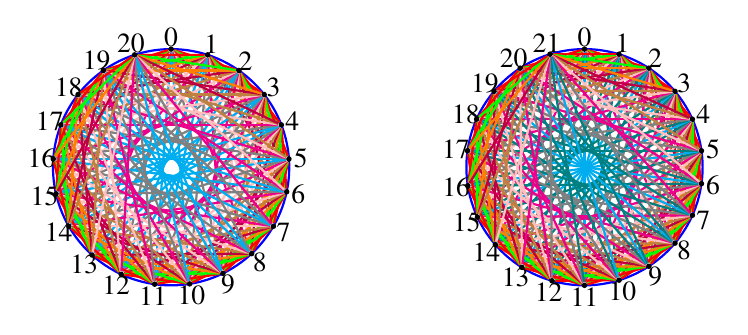
\begin{tikzpicture}[scale=1.5,
        dot/.style={circle, fill=black, minimum size=2pt, inner sep=0pt},
        lbl/.style={draw=none, fill=none, inner sep=0pt, anchor=center}
      ]
  
          \draw[blue, thick] (0,0) circle (1);
          \foreach \i in {0,...,20} {
            \pgfmathtruncatemacro{\angle}{90 - \i*360/21}
            \node[dot] (a\i) at (\angle:1) {};
            \node[lbl] at (\angle:1.1) {\i};
          }
          \foreach \i in {0,...,20} {
            \foreach \j in {0,...,20} {
              \ifnum\j>\i\relax
                \pgfmathtruncatemacro{\d}{mod(\j-\i,21)}
                \pgfmathtruncatemacro{\dmin}{min(\d,21-\d)}
                %\ifnum\dmin=1   \draw[blue,   thick] (a\i) -- (a\j); \fi
                \ifnum\dmin=2   \draw[red,    thick] (a\i) -- (a\j); \fi
                \ifnum\dmin=3   \draw[green,  thick] (a\i) -- (a\j); \fi
                \ifnum\dmin=4   \draw[orange, thick] (a\i) -- (a\j); \fi
                \ifnum\dmin=5   \draw[purple, thick] (a\i) -- (a\j); \fi
                \ifnum\dmin=6   \draw[brown,  thick] (a\i) -- (a\j); \fi
                \ifnum\dmin=7   \draw[pink,   thick] (a\i) -- (a\j); \fi
                \ifnum\dmin=8   \draw[magenta,thick] (a\i) -- (a\j); \fi
                \ifnum\dmin=9   \draw[gray,   thick] (a\i) -- (a\j); \fi
                \ifnum\dmin=10  \draw[cyan,   thick] (a\i) -- (a\j); \fi
              \fi
            }
          }
  
        % K_22
        \begin{scope}[shift={(3.5,0)}]
          \draw[blue, thick] (0,0) circle (1);
          \foreach \i in {0,...,21} {
            \pgfmathtruncatemacro{\angle}{90 - \i*360/22}
            \node[dot] (b\i) at (\angle:1) {};
            \node[lbl] at (\angle:1.1) {\i};
          }
          \foreach \i in {0,...,21} {
            \foreach \j in {0,...,21} {
              \ifnum\j>\i\relax
                \pgfmathtruncatemacro{\d}{mod(\j-\i,22)}
                \pgfmathtruncatemacro{\dmin}{min(\d,22-\d)}
                %\ifnum\dmin=1   \draw[blue,   thick] (b\i) -- (b\j); \fi
                \ifnum\dmin=2   \draw[red,    thick] (b\i) -- (b\j); \fi
                \ifnum\dmin=3   \draw[green,  thick] (b\i) -- (b\j); \fi
                \ifnum\dmin=4   \draw[orange, thick] (b\i) -- (b\j); \fi
                \ifnum\dmin=5   \draw[purple, thick] (b\i) -- (b\j); \fi
                \ifnum\dmin=6   \draw[brown,  thick] (b\i) -- (b\j); \fi
                \ifnum\dmin=7   \draw[pink,   thick] (b\i) -- (b\j); \fi
                \ifnum\dmin=8   \draw[magenta,thick] (b\i) -- (b\j); \fi
                \ifnum\dmin=9   \draw[gray,   thick] (b\i) -- (b\j); \fi
                \ifnum\dmin=10  \draw[teal,   thick] (b\i) -- (b\j); \fi
                \ifnum\dmin=11  \draw[cyan,   thick] (b\i) -- (b\j); \fi
              \fi
            }
          }
        \end{scope}
  
      \end{tikzpicture}
    \end{center}
    \caption{[1] $K_{21}$ (left) and $K_{22}$ (right) with edges colored by length.}
    \label{fig:K21K22colored}
  \end{figure}
$K_{21}$ has lengths $\{1,\hdots, 10\}$ has lengths in $\{1,\hdots, 10\}\sqcup \{\infty\}$. For even cases of $n$, we turn the largest length and largest node label into $\infty$, which requires a lot of background to understand. Instead of explaining it all, just know that we take $V(K_{22})$ to be $\ZZ_{21}\sqcup \{\infty\}$ and that we define development and length as follows for it. $$\ell_{22}(uv)=\begin{cases}\min\{|u-v|,21-|u-v|\}, & u,v\neq \infty, \\ \infty, & u\text{ or }v=\infty \end{cases} \text{ and }v\mapsto 
  \begin{cases}
    v+1,&v\in\mathbb{Z}_{n-1},\\
    \infty,        &v=\infty.
  \end{cases}$$
Ok, now the issue is that $P_{3}\sqcup S_{6}$ only has $7$ edges... we can't fit $10$ or $11$ lengths onto its $7$ edges! So then of course we cant just generate all edges of $K_{21}$ or $K_{22}$ with one labeling. So we take care of lengths $1,2,3$ and $1,2,3,\infty$ for $K_{21}$ and $K_{22}$, respectively, and then use some variation of $\sigma^{+-}$ to generate the remaining sets of $7$ lengths. To begin this, we define a new edge length.
  $$\ell_{7}^{+}(uv)=\begin{cases} u+v\textbf{ mod }7, & u,v\neq \infty,\\ v, &u=\infty. \end{cases}$$
For any edge $uv$ of length $l\in \{1,\hdots, 10\}\sqcup \{\infty\}$, notice that $\ell^{+}_{7}(uv)\in \ZZ_{7}$, obviously. So then instead of one generator, where each edge has distinct length $\ell_{21}$ or $\ell_{22}$, respectively, we use a $\lambda_{7}$-labeling of $P_{3}\sqcup S_{6}$ and a $\lambda_{8}$ labeling of $P_{3}\sqcup S_{6}$, respectively, which is defined below.
\begin{definition}[Banegas, Freyberg]
A $\lambda_{r}$-labeling of an $m$-edge graph $G$ where $r$ is idempotent in $\ZZ_{2m}$, is $k=\floor{\frac{r}{2}}$ concurrent injections $f_{1},\hdots, f_{k}:\begin{cases} \ZZ_{2m+r}\to V(G)\text{, } r\text{ is odd}\\ \ZZ_{2m+r-1}\cup \{\infty\}\to V(G) \text{, } r\text{ is even}\end{cases}$ where $L=\begin{cases} [k]\text{, }r\text{ is odd},\\ [k-1]\cup \{\infty\}\text{, }r\text{ is even}\end{cases}$ is the set of all permitted standard $\ell_{2m}$-lengths found in any labeling, where the following holds.

Let $G_{i}$ be the copy of $G$ obtained via $f_{i}$, then in the set of all labeled copies $\{G_{1},\hdots,G_{k}\}$ of $G$ given given by $\lambda_{r}$, we have that 
\begin{align*}
&\text{All edges have $\ell_{2m}$ lengths in } [k]\text{ or }[k-1]\cup \{\infty\},\text{ for odd and even cases, respectively.}\\
&\text{All generators are pairwise }\ell_{2m}\times \ell^{+}_{m}\text{-edge disjoint}\\
&\text{Some generator contains an edge $e$ of length pair }(\ell_{2m}(e),\ell^{+}_{m}(e)(e))=(a,b)\text{ for each }(a,b)\in L\times \ZZ_{m}
\end{align*}
\end{definition}
This labeling gives us the following theorem, which mentions a labeling called $\rho^{+}$. This is just a weaker version of $\sigma^{+-}$, which itself is a special type of $\rho^{+}$-labeling.
\begin{thm}[Banegas, Freyberg]
If an $m$-edge graph $G$ admits a $\lambda_{r}$-labeling and a $\rho^{+-}$-labeling, then there exists a $G$-decomposition of $K_{2mt+r}$ for all $t\geq 1$.
\end{thm}
Alright... that was a lot. The point is, now for $K_{2mt+r}$ whose base graph $K_{2m+r}$ has more edge lengths than $G$ has edges (it will have $m+k$ distinct lengths where $k=\floor{\frac{r}{2}}$), we can use this new $\lambda_{r}$-labeling. These labeling will generate all edges of lengths in $[k]$ if $r$ is odd or $[k-1]\cup \{\infty\}$ if $r$ is even, when developed by $7$. That is, if $\lambda_{r}(G)$ gives us $\{G_{i}\mid i\in \ZZ_{k}\}$, then for each $t\geq 1$, through the action 
$$\langle 7\rangle_{+}\curvearrowright S(K_{2mt+r})\text{ via }i(G)\coloneq (V(G),E(G))\mapsto (V(G)+i,E(G)+ii),\,\forall G\in S(K_{2mt+r})\text{ and }\forall i\in \langle 7\rangle_{+},$$
all edges $E_{L}$ of $K_{2mt+r}$ with standard $\ell_{2mt+r}$-length in $L$ ($[k],[k-1]\cup \{\infty\}$ for $r$ odd, even, respectively), will appear in some copy of $G$ in the union $\bigcup_{i\in [k]}\mathrm{Orb}_{\langle 7\rangle_{+}}(G_{i})$ of all orbits of the $\lambda_{r}$-labeling of $G$. This leaves us with all edges with lengths in $[m+k]\setminus [k]$, which has size $m$. We can modify a $\sigma^{+-}$-labeling to collect these remaining edges. If $G^{*}_{0}$ is a $\sigma^{+-}$-labeled copy of $G$, where $A\sqcup B$ is it's defining ordered-bipartition, then let $G_{0,j}$ be the labeling obtained by only developing the $B$ nodes by $k+7j$ for each $j\in \ZZ_{k-1}$. We have that 
$$\GG=(\bigcup_{i\in [k]}\mathrm{Orb}_{\langle 7\rangle_{+}}(G_{i}))\cup (\bigcup_{j\in [t]}\mathrm{Orb}_{\ZZ_{2mt+r}}(G_{0,j}))\text{ is a is a $G$-decomposition of $K_{2mt+r}$.}$$


  \begin{figure}[H]
    \begin{center}
      
      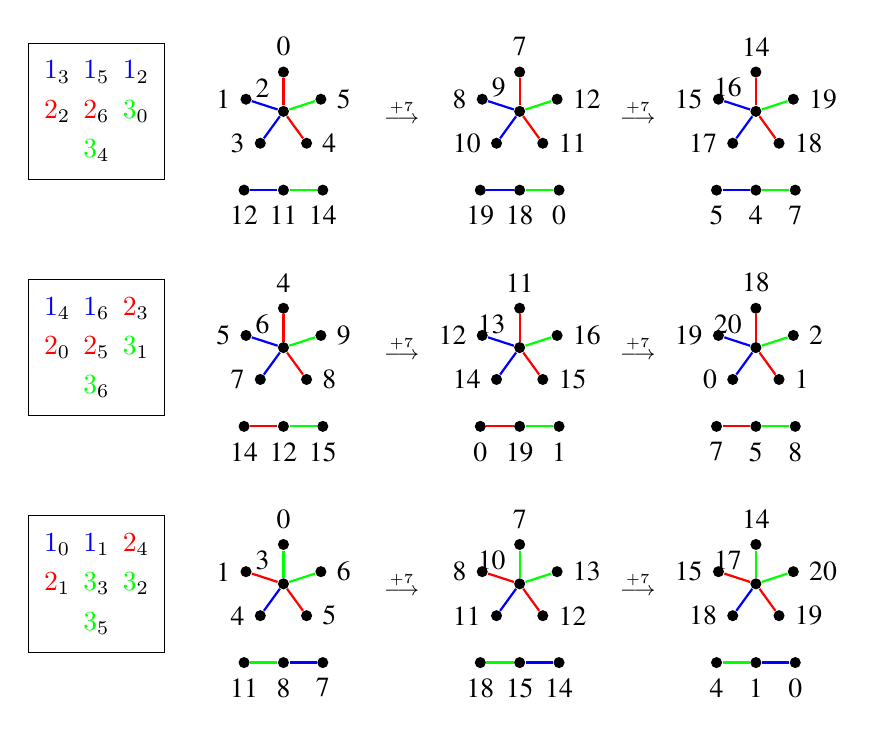
\begin{tikzpicture}[scale=1]
        %-----------------------------------------column 1----------------------------------------------------------------
        \tikzset{
            dot/.style={circle, fill=black, minimum size=4pt, inner sep=0pt},
            lbl/.style={draw=none, fill=none, inner sep=0pt, anchor=center}
          }
        % — Labeling 1 —
        \begin{scope}
          \matrix (arr1) [draw,
                          anchor=east,
                          matrix of nodes,
                          nodes={minimum size=0.5cm, inner sep=0pt, anchor=center}
                         ] at (-1.5,0) {
            $\textcolor{blue}{1}_{3}$ & $\textcolor{blue}{1}_{5}$ & $\textcolor{blue}{1}_{2}$ \\
            $\textcolor{red}{2}_{2}$  & $\textcolor{red}{2}_{6}$  & $\textcolor{green}{3}_{0}$ \\
                                      & $\textcolor{green}{3}_{4}$ &                      \\
          };
  
          \node[dot,label=above left:2] (C1)  at (0,0)    {};
          \node[dot,label=above:0]      (L10) at (90:0.5)  {};
          \node[dot,label=left:1]       (L11) at (162:0.5){};
          \node[dot,label=left:3]       (L13) at (234:0.5){};
          \node[dot,label=right:4]      (L14) at (306:0.5){};
          \node[dot,label=right:5]      (L15) at (18:0.5) {};
  
          \draw[red,   thick]   (C1) -- (L10);
          \draw[blue,  thick]   (C1) -- (L11);
          \draw[blue,  thick]   (C1) -- (L13);
          \draw[red,   thick]   (C1) -- (L14);
          \draw[green, thick]   (C1) -- (L15);
  
          \node[dot,label=below:12] (P12) at (-0.5,-1) {};
          \node[dot,label=below:11] (P11) at ( 0  ,-1) {};
          \node[dot,label=below:14] (P14) at ( 0.5,-1) {};
  
          \draw[blue,  thick] (P12) -- (P11);
          \draw[green, thick] (P11) -- (P14);

          \node at (1.5,0) {\scriptsize $\overset{+7}{\longrightarrow}$};

        \end{scope}
  
        % — Labeling 2 —
        \begin{scope}[yshift=-3cm]
          \matrix (arr2) [draw,
                          anchor=east,
                          matrix of nodes,
                          nodes={minimum size=0.5cm, inner sep=0pt, anchor=center}
                         ] at (-1.5,0) {
            $\textcolor{blue}{1}_{4}$ & $\textcolor{blue}{1}_{6}$ & $\textcolor{red}{2}_{3}$ \\
            $\textcolor{red}{2}_{0}$  & $\textcolor{red}{2}_{5}$  & $\textcolor{green}{3}_{1}$ \\
                                      & $\textcolor{green}{3}_{6}$ &                      \\
          };
  
          \node[dot,label=above left:6] (C2)  at (0,0)    {};
          \node[dot,label=above:4]      (L24) at (90:0.5)  {};
          \node[dot,label=left:5]       (L25) at (162:0.5){};
          \node[dot,label=left:7]       (L27) at (234:0.5){};
          \node[dot,label=right:8]      (L28) at (306:0.5){};
          \node[dot,label=right:9]      (L29) at (18:0.5) {};
  
          \draw[red,   thick]   (C2) -- (L24);
          \draw[blue,  thick]   (C2) -- (L25);
          \draw[blue,  thick]   (C2) -- (L27);
          \draw[red,   thick]   (C2) -- (L28);
          \draw[green, thick]   (C2) -- (L29);
  
          \node[dot,label=below:14] (P214) at (-0.5,-1) {};
          \node[dot,label=below:12] (P212) at ( 0  ,-1) {};
          \node[dot,label=below:15] (P215) at ( 0.5,-1) {};
  
          \draw[red,   thick]   (P214) -- (P212);
          \draw[green, thick]   (P212) -- (P215);
          \node at (1.5,0) {\scriptsize $\overset{+7}{\longrightarrow}$};
        \end{scope}
  
        % — Labeling 3 —
        \begin{scope}[yshift=-6cm]
          \matrix (arr3) [draw,
                          anchor=east,
                          matrix of nodes,
                          nodes={minimum size=0.5cm, inner sep=0pt, anchor=center}
                         ] at (-1.5,0) {
            $\textcolor{blue}{1}_{0}$ & $\textcolor{blue}{1}_{1}$ & $\textcolor{red}{2}_{4}$ \\
            $\textcolor{red}{2}_{1}$  & $\textcolor{green}{3}_{3}$ & $\textcolor{green}{3}_{2}$ \\
                                      & $\textcolor{green}{3}_{5}$ &                      \\
          };
  
          \node[dot,label=above left:3] (C3)  at (0,0)    {};
          \node[dot,label=above:0]      (L30) at (90:0.5)  {};
          \node[dot,label=left:1]       (L31) at (162:0.5){};
          \node[dot,label=left:4]       (L34) at (234:0.5){};
          \node[dot,label=right:5]      (L35) at (306:0.5){};
          \node[dot,label=right:6]      (L36) at (18:0.5) {};
  
          \draw[green, thick]   (C3) -- (L30);
          \draw[red,   thick]   (C3) -- (L31);
          \draw[blue,  thick]   (C3) -- (L34);
          \draw[red,   thick]   (C3) -- (L35);
          \draw[green, thick]   (C3) -- (L36);
  
          \node[dot,label=below:11] (P311) at (-0.5,-1) {};
          \node[dot,label=below:8]  (P38)  at ( 0  ,-1) {};
          \node[dot,label=below:7]  (P37)  at ( 0.5,-1) {};
  
          \draw[green, thick] (P311) -- (P38);
          \draw[blue,  thick] (P38)  -- (P37);
          \node at (1.5,0) {\scriptsize $\overset{+7}{\longrightarrow}$};
        \end{scope}

        %-------------------------------------------column2-----------------------------------------------------------------
        % — Labeling 1 —
        \begin{scope}[shift={(3,0)}]
            \node[dot,label=above left:9] (C1)  at (0,0)    {};
          \node[dot,label=above:7]      (L10) at (90:0.5)  {};
          \node[dot,label=left:8]       (L11) at (162:0.5){};
          \node[dot,label=left:10]       (L13) at (234:0.5){};
          \node[dot,label=right:11]      (L14) at (306:0.5){};
          \node[dot,label=right:12]      (L15) at (18:0.5) {};
  
          \draw[red,   thick]   (C1) -- (L10);
          \draw[blue,  thick]   (C1) -- (L11);
          \draw[blue,  thick]   (C1) -- (L13);
          \draw[red,   thick]   (C1) -- (L14);
          \draw[green, thick]   (C1) -- (L15);
  
          \node[dot,label=below:19] (P12) at (-0.5,-1) {};
          \node[dot,label=below:18] (P11) at ( 0  ,-1) {};
          \node[dot,label=below:0] (P14) at ( 0.5,-1) {};
  
          \draw[blue,  thick] (P12) -- (P11);
          \draw[green, thick] (P11) -- (P14);
          \node at (1.5,0) {\scriptsize $\overset{+7}{\longrightarrow}$};
        \end{scope}

        % — Labeling 2 —
        \begin{scope}[shift={(3,-3)}]
            \node[dot,label=above left:13] (C2)  at (0,0)    {};
            \node[dot,label=above:11]      (L24) at (90:0.5)  {};
            \node[dot,label=left:12]       (L25) at (162:0.5){};
            \node[dot,label=left:14]       (L27) at (234:0.5){};
            \node[dot,label=right:15]      (L28) at (306:0.5){};
            \node[dot,label=right:16]      (L29) at (18:0.5) {};
    
            \draw[red,   thick]   (C2) -- (L24);
            \draw[blue,  thick]   (C2) -- (L25);
            \draw[blue,  thick]   (C2) -- (L27);
            \draw[red,   thick]   (C2) -- (L28);
            \draw[green, thick]   (C2) -- (L29);
    
            \node[dot,label=below:0] (P214) at (-0.5,-1) {};
            \node[dot,label=below:19] (P212) at ( 0  ,-1) {};
            \node[dot,label=below:1] (P215) at ( 0.5,-1) {};
    
            \draw[red,   thick]   (P214) -- (P212);
            \draw[green, thick]   (P212) -- (P215);
            \node at (1.5,0) {\scriptsize $\overset{+7}{\longrightarrow}$};
            \end{scope}

            % — Labeling 3 —
            \begin{scope}[shift={(3,-6)}]
                \node[dot,label=above left:10] (C3)  at (0,0)    {};
                \node[dot,label=above:7]      (L30) at (90:0.5)  {};
                \node[dot,label=left:8]       (L31) at (162:0.5){};
                \node[dot,label=left:11]       (L34) at (234:0.5){};
                \node[dot,label=right:12]      (L35) at (306:0.5){};
                \node[dot,label=right:13]      (L36) at (18:0.5) {};
        
                \draw[green, thick]   (C3) -- (L30);
                \draw[red,   thick]   (C3) -- (L31);
                \draw[blue,  thick]   (C3) -- (L34);
                \draw[red,   thick]   (C3) -- (L35);
                \draw[green, thick]   (C3) -- (L36);
        
                \node[dot,label=below:18] (P311) at (-0.5,-1) {};
                \node[dot,label=below:15]  (P38)  at ( 0  ,-1) {};
                \node[dot,label=below:14]  (P37)  at ( 0.5,-1) {};
        
                \draw[green, thick] (P311) -- (P38);
                \draw[blue,  thick] (P38)  -- (P37);
                \node at (1.5,0) {\scriptsize $\overset{+7}{\longrightarrow}$};
                \end{scope}

        %-------------------------------------------column2-----------------------------------------------------------------
            % — Labeling 1 —
            \begin{scope}[shift={(6,0)}]
                \node[dot,label=above left:16] (C1)  at (0,0)    {};
                \node[dot,label=above:14]      (L10) at (90:0.5)  {};
                \node[dot,label=left:15]       (L11) at (162:0.5){};
                \node[dot,label=left:17]       (L13) at (234:0.5){};
                \node[dot,label=right:18]      (L14) at (306:0.5){};
                \node[dot,label=right:19]      (L15) at (18:0.5) {};

                \draw[red,   thick]   (C1) -- (L10);
                \draw[blue,  thick]   (C1) -- (L11);
                \draw[blue,  thick]   (C1) -- (L13);
                \draw[red,   thick]   (C1) -- (L14);
                \draw[green, thick]   (C1) -- (L15);

                \node[dot,label=below:5] (P12) at (-0.5,-1) {};
                \node[dot,label=below:4] (P11) at ( 0  ,-1) {};
                \node[dot,label=below:7] (P14) at ( 0.5,-1) {};

                \draw[blue,  thick] (P12) -- (P11);
                \draw[green, thick] (P11) -- (P14);
            \end{scope}

            % — Labeling 2 —
            \begin{scope}[shift={(6,-3)}]
                \node[dot,label=above left:20] (C2)  at (0,0)    {};
                \node[dot,label=above:18]      (L24) at (90:0.5)  {};
                \node[dot,label=left:19]       (L25) at (162:0.5){};
                \node[dot,label=left:0]       (L27) at (234:0.5){};
                \node[dot,label=right:1]      (L28) at (306:0.5){};
                \node[dot,label=right:2]      (L29) at (18:0.5) {};

                \draw[red,   thick]   (C2) -- (L24);
                \draw[blue,  thick]   (C2) -- (L25);
                \draw[blue,  thick]   (C2) -- (L27);
                \draw[red,   thick]   (C2) -- (L28);
                \draw[green, thick]   (C2) -- (L29);

                \node[dot,label=below:7] (P214) at (-0.5,-1) {};
                \node[dot,label=below:5] (P212) at ( 0  ,-1) {};
                \node[dot,label=below:8] (P215) at ( 0.5,-1) {};

                \draw[red,   thick]   (P214) -- (P212);
                \draw[green, thick]   (P212) -- (P215);
                \end{scope}

                % — Labeling 3 —
                \begin{scope}[shift={(6,-6)}]
                    \node[dot,label=above left:17] (C3)  at (0,0)    {};
                    \node[dot,label=above:14]      (L30) at (90:0.5)  {};
                    \node[dot,label=left:15]       (L31) at (162:0.5){};
                    \node[dot,label=left:18]       (L34) at (234:0.5){};
                    \node[dot,label=right:19]      (L35) at (306:0.5){};
                    \node[dot,label=right:20]      (L36) at (18:0.5) {};
            
                    \draw[green, thick]   (C3) -- (L30);
                    \draw[red,   thick]   (C3) -- (L31);
                    \draw[blue,  thick]   (C3) -- (L34);
                    \draw[red,   thick]   (C3) -- (L35);
                    \draw[green, thick]   (C3) -- (L36);
            
                    \node[dot,label=below:4] (P311) at (-0.5,-1) {};
                    \node[dot,label=below:1]  (P38)  at ( 0  ,-1) {};
                    \node[dot,label=below:0]  (P37)  at ( 0.5,-1) {};
            
                    \draw[green, thick] (P311) -- (P38);
                    \draw[blue,  thick] (P38)  -- (P37);
                    \end{scope}



      \end{tikzpicture}
    \end{center}
    \caption{[1] A $\lambda_{7}$-labeling of $P_{3}\sqcup S_{6}$ (left column) that generates all edges of lengths $1,2,\text{ and }3$ in $K_{21}$ when developed by $7$.}
    \label{fig:K21labelingex}
  \end{figure}
The union $\bigcup_{i\in [k]}\mathrm{Orb}_{\langle 7\rangle_{+}}(G_{i})$ of all orbits shown above will give us all edges of $K_{14t+7}$ with lengths in $\{1,2,3\}$. At each step $t\mapsto t+1$, the orbits just grow with the complete graph's order. and then the remaining lengths $\{4,\hdots, 10\}$ can be generated by a modified $\sigma^{+-}$-labeling (a $\rho^{+}$-labeling). 

A similar strategy can be used for $K_{22}$ and it turns out that the existence of a $\lambda_{7}$ and $\lambda_{8}$ labeling of $P_{3}\sqcup S_{6}$ along with the existence of a $\rho^{+}$-labeling of $P_{3}\sqcup S_{6}$ proved that it decomposes $K_{14t+7}$ and $K_{14t+8}$ for all $t\geq 1$. An important note about this type of labeling, it has no bipartite condition. So this strategy could in theory be used for any small graph, but then you could not use $\rho^{+}$ to clean up the remaining edge lengths.
\section{Summary}
In the Thesis, \textit{Seven Edge Forest Designs}, by Banegas and Freyberg, they prove that there exists a $7$-edge forest decomposition of $K_{n}$ if and only if $n\equiv 0,1,7,\text{or }8\pmod {14}$ using $\sigma^{+-}$-labelings, $\lambda$-labelings along with a different construction for the exceptional graph $P_{2}\sqcup S_{7}$. In this write up, the core machinery and intuition guiding this work was covered. 

Ideas not covered here were many particulars about creating new labeling techniques, the exceptional graph construction, some general results of Galaxy Decompositions of Complete Bipartites, some new wraparound edge mappings that preserve length, a new graphical interface for NetworkX graphs called \textit{Tikzgrapher} developed by Banegas in Python, and a section on pairing \textit{Tikzgrapher} with some constraint programming libraries to find $\sigma^{+-}$ and $\lambda$ labelings. We now cite the thesis below and then move onto some exercises.

\noindent
[1] D.~M.~Banegas, \emph{Seven Edge Forest Designs}, Master’s thesis,
University of Minnesota Duluth, 2025.
\bibliographystyle{plain}
\bibliography{refs} % uncomment if using BibTeX
\newpage
\section{Exercises}

$\mathbf{(1)}$ Find a $\sigma^{+-}$-labeling of $S_{4}\sqcup P_{5}$ and create a diagram showing each step in generating it's orbit via the group action defined in the \textbf{Intuition} section replacing $\ZZ_{5}$ with $\ZZ_{14}$ (\textit{develop} by $1$ or add $1$ modulo $14$ to all of it's nodes repeatedly). How many copies of $S_{4}\sqcup P_{5}$ appear in the $S_{4}\sqcup P_{5}$-decomposition of $K_{14}$ generated by this labeling?

Hint: label the nodes from $\{0,1,\hdots, 11, 12\}$ so that (i) every node $u$ either belongs to $A$ or $B$ where all nodes in $A$ are smaller than their neighbors, and all nodes in $B$ are larger than their neighbors (ii) Each set of neighbors gives has a unique difference $|a-b|=b-a\in [7]$. Then (iii) develop the resulting labeling by $1$ modulo $14$ repeatedly to get its orbit.
\newpage
$\mathbf{(2)}$ Find a $\lambda_{7}$-labeling and $\lambda_{8}$-labeling of $S_{4}\sqcup P_{5}$, and show the orbits of each of it's generators via the group action defined in \textbf{Intuition} section replacing $\ZZ_{5}$ with $\langle 7\rangle_{+} < \ZZ_{21}$. Here are steps to do this:

(a) Label $3$ copies of $S_{4}\sqcup P_{5}$ from $\ZZ_{21}$ such that: 
\begin{itemize}
\item  No two copies have edges of the same length pair $\ell_{21}\times \ell^{+}_{7}(uv)\coloneq (\min\{21-|u-v|,|u-v|\},u+v\pmod{7})$
\item For every length $l\in \{1,2,3\}$ we can find an edge of length pair $(l,i)$ for each $i\in \ZZ_{7}$
\end{itemize}
Repeat this for $\lambda_{8}$ using vertex labels from $\ZZ_{21}\cup \{\infty\}$ and with lengths $\{1,2,3,\infty\}$ using the modified length definitions from the \textbf{$\lambda$-labelings} section.

(b) Develop your labelings by $7$ modulo $21$ repeatedly to find the orbits for your $\lambda_{7}$ and $\lambda_{8}$ labelings. What could we do to the $\sigma^{+-}$-labeling of this graph to collect the remaining edges of $K_{21}$?

\end{document}
